%%%%%%%%%%%%%%%%%%%%%%%%%%%%%%%%%%%%%%%%%%%%%%%%%%%%%%%%%%%%%%%%%%%%%%%%%%%%%%%
% Definici�n del tipo de documento.                                           %
% Posibles tipos de papel: a4paper, letterpaper, legalpapper                  %
% Posibles tama�os de letra: 10pt, 11pt, 12pt                                 %
% Posibles clases de documentos: article, report, book, slides                %
%%%%%%%%%%%%%%%%%%%%%%%%%%%%%%%%%%%%%%%%%%%%%%%%%%%%%%%%%%%%%%%%%%%%%%%%%%%%%%%
\documentclass[a4paper,10pt]{article}


%%%%%%%%%%%%%%%%%%%%%%%%%%%%%%%%%%%%%%%%%%%%%%%%%%%%%%%%%%%%%%%%%%%%%%%%%%%%%%%
% Los paquetes permiten ampliar las capacidades de LaTeX.                     %
%%%%%%%%%%%%%%%%%%%%%%%%%%%%%%%%%%%%%%%%%%%%%%%%%%%%%%%%%%%%%%%%%%%%%%%%%%%%%%%

% Paquete para inclusi�n de gr�ficos.
\usepackage{graphicx}

% Paquete para definir la codificaci�n del conjunto de caracteres usado
% (latin1 es ISO 8859-1).
\usepackage[latin1]{inputenc}

% Paquete para definir el idioma usado.
\usepackage[spanish]{babel}

\usepackage{multirow} 

%\usepackage{multicolumn} 

% T�tulo principal del documento.
\title{		\textbf{Trabajo pr�ctico 0: Infraestructura b�sica}}

% Informaci�n sobre los autores.
\author{	Alejandro Garc�a Marra, \textit{Padr�n Nro. 91.516}                     \\
            \texttt{ alemarra@gmail.com }                                              \\
            Sebasti�n Javier Bogado, \textit{Padr�n Nro. 91.707}                     \\
            \texttt{ sebastian.j.bogado@gmail.com }                                              \\
            \normalsize{Grupo Nro. 0 - 2do. Cuatrimestre de 2012}                       \\
            \normalsize{66.20 Organizaci�n de Computadoras}                             \\
            \normalsize{Facultad de Ingenier�a, Universidad de Buenos Aires}            \\
       }
\date{}



\begin{document}

% Inserta el t�tulo.
\maketitle

% Quita el n�mero en la primer p�gina.
\thispagestyle{empty}

% Resumen
\begin{abstract}

El presente trabajo busca crear un programa que permita el ordenamiento de archivos a trav�s de dos implementaciones distintas, una utilizando el algoritmo Quicksort y la otra el algoritmo Stooge sort.\\
Sobre este programa, luego, se realizar�n una serie de mediciones con el fin de determinar los desempe�os relativos de cada implementaci�n y las posibles mejoras a realizar. 
Para esto haremos uso de los programas \textbf{time} y \textbf{gprof}.

\end{abstract}


\section{Introducci�n}

Algo sobre profiling?

\newpage

\section{Mediciones}

\subsection{Valores Obtenidos}

En la tabla~\ref{tab001} se presentan las mediciones realizadas con \textbf{time} sobre ambos algoritmos de ordenamiento y con archivos de distintos tama�os.\\

Adem�s de los archivos indicados en el enunciado, fueron agregadas mediciones sobre archivos con tama�os arbitrarios, mayores, con el fin de mostrar de mejor manera las diferencias entre algoritmos.

\begin{table}[!htp]
\begin{center}
\begin{tabular}{cc|c|c|c|c|c|c|} 
\cline{3-8}
& & \multicolumn{3}{ c|}{Quicksort} & \multicolumn{3}{c|}{Stooge sort}\\ \cline{3-8}
&   & Ordenado & Invertido & Aleatorio & Ordenado & Invertido & Aleatorio \\ \cline{1-8}
\multicolumn{1}{|c}{\multirow{3}{*}{1kb}} &
\multicolumn{1}{|c|}{real$^{*}$} & 0.00 & 0.00 &0.00 & 0.00 & 0.00 & 0.00 \\ \cline{2-8}
\multicolumn{1}{|c}{}                        &
\multicolumn{1}{|c|}{user$^{*}$} & 0.00 & 0.00 &0.00 & 0.00 & 0.00 & 0.00 \\ \cline{2-8}
\multicolumn{1}{|c}{}                        &
\multicolumn{1}{|c|}{sys$^{*}$} & 0.00 & 0.00 &0.00 & 0.00 & 0.00 & 0.00 \\ \cline{1-8}
\multicolumn{1}{|c}{\multirow{3}{*}{8kb}} &
\multicolumn{1}{|c|}{real} & 0.00 & 0.00 &0.00 & 0.02 & 0.02 & 0.01 \\ \cline{2-8}
\multicolumn{1}{|c}{}                        &
\multicolumn{1}{|c|}{user} & 0.00 & 0.00 &0.00 & 0.01 & 0.01 & 0.01 \\ \cline{2-8}
\multicolumn{1}{|c}{}                        &
\multicolumn{1}{|c|}{sys} & 0.00 & 0.00 &0.00 & 0.00 & 0.00 & 0.00 \\ \cline{1-8}
\multicolumn{1}{|c}{\multirow{3}{*}{16kb}} &
\multicolumn{1}{|c|}{real} & 0.00 & 0.00 &0.00 & 0.00 & 0.02 & 0.02 \\ \cline{2-8}
\multicolumn{1}{|c}{}                        &
\multicolumn{1}{|c|}{user} & 0.00 & 0.00 &0.00 & 0.00 & 0.01 & 0.02 \\ \cline{2-8}
\multicolumn{1}{|c}{}                        &
\multicolumn{1}{|c|}{sys} & 0.00 & 0.00 &0.00 & 0.00 & 0.00 & 0.00 \\ \cline{1-8}
\multicolumn{1}{|c}{\multirow{3}{*}{32kb}} &
\multicolumn{1}{|c|}{real} & 0.00 & 0.00 &0.00 & 0.17 & 0.17 & 0.17 \\ \cline{2-8}
\multicolumn{1}{|c}{}                        &
\multicolumn{1}{|c|}{user} & 0.00 & 0.00 &0.00 & 0.17 & 0.17 & 0.17 \\ \cline{2-8}
\multicolumn{1}{|c}{}                        &
\multicolumn{1}{|c|}{sys} & 0.00 & 0.00 &0.00 & 0.00 & 0.00 & 0.00 \\ \cline{1-8}
\multicolumn{1}{|c}{\multirow{3}{*}{64kb}} &
\multicolumn{1}{|c|}{real} & 0.00 & 0.00 &0.00 & 1.44 & 1.44 & 1.44 \\ \cline{2-8}
\multicolumn{1}{|c}{}                        &
\multicolumn{1}{|c|}{user} & 0.00 & 0.00 &0.00 & 1.44 & 1.43 & 1.44 \\ \cline{2-8}
\multicolumn{1}{|c}{}                        &
\multicolumn{1}{|c|}{sys} & 0.00 & 0.00 &0.00 & 0.00 & 0.00 & 0.00 \\ \cline{1-8}
\multicolumn{1}{|c}{\multirow{3}{*}{1024kb}} &
\multicolumn{1}{|c|}{real} & 0.04 & 0.03 &0.03 & $>$1500 & $>$1500 & $>$1500 \\ \cline{2-8}
\multicolumn{1}{|c}{}                        &
\multicolumn{1}{|c|}{user} & 0.03 & 0.02 &0.03 & $>$1500 & $>$1500 & $>$1500 \\ \cline{2-8}
\multicolumn{1}{|c}{}                        &
\multicolumn{1}{|c|}{sys} & 0.00 & 0.00 &0.00 & 0.00 & 0.00 & 0.00 \\ \cline{1-8}
\end{tabular}
\caption{Resultados comando Time } \label{tab001}
\end{center}
\end{table}

$^{*}$ Referencia: 
\begin{itemize}
 \item real: \%e, tiempo total real usado por el proceso.
 \item user: \%U, total de segundos-CPU usados por el proceso directamente.
 \item sys : \%S, total de segundos-CPU utilizados por el systema en nombre del proceso.
\end{itemize}



\subsection{An�lisis de los datos}

La marcada diferencia entre la complejidad de los algoritmos se refleja en muestras tan chicas como la de 8kb. 
A partir de ah�, el Stooge sort ya hace suficiente uso del procesador como para ser notado por time, mientras que el Quicksort hace lo propio reci�n en la muestra m�s grande, de 1024kb. En este caso, el Stooge sort se torn� intolerable.

En la figura~\ref{fig001} se muestra el gr�fico del tiempo insumido por el Quicksort para las distintas muestras.\\
En la figura~\ref{fig002} se muestra el gr�fico del tiempo insumido por el Stooge sort para las distintas muestras, a excepci�n de la de 1024kb, porque demanda una escala que har�a inapreciable la situaci�n de las otras muestras.

\begin{figure}[!htp]
\begin{center}
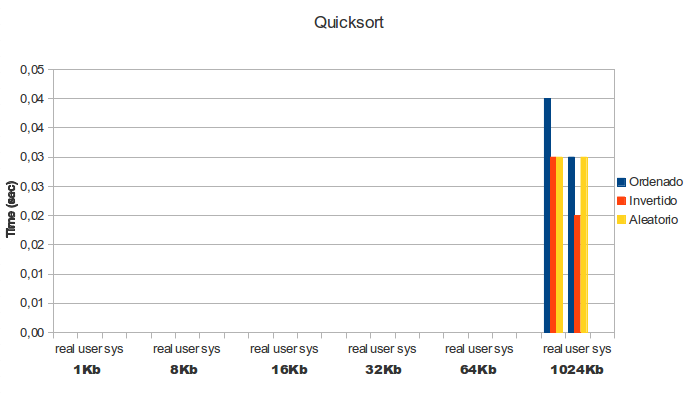
\includegraphics[width=1\textwidth]{quicksort.png}
\end{center}
\caption{Tiempo tomado para distintas muestras del Quicksort.} \label{fig001}
\end{figure}

\begin{figure}[!htp]
\begin{center}
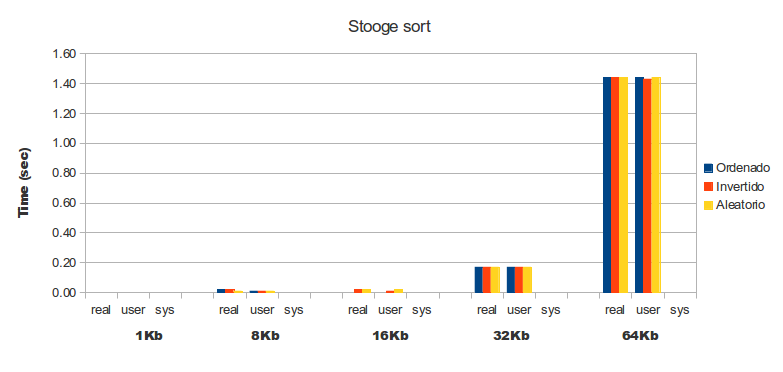
\includegraphics[width=1.1\textwidth]{stoogesort.png}
\end{center}
\caption{Tiempo tomado para distintas muestras del Stooge sort.} \label{fig002}
\end{figure}



Gr�fico de speedup, quick vs stooge

\newpage

\section{Profiling}

Para realizar el profiling tomamos una muestra suficientemente grande como para que las funciones mismas de \textbf{gprof} tuvieran una incidencia despreciable en la prueba. 
En la figura~\ref{fig003} se muestra un ejemplo de c�mo presentar las ilustraciones del informe.

% Inclusi�n de una imagen en formato EPS (Encapsulated Postscript).
\begin{figure}[!htp]
\begin{center}
%\includegraphics[width=0.5\textwidth]{fig001.eps}
\end{center}
\caption{Facultad de Ingenier�a $-$ Universidad de Buenos Aires.} \label{fig003}
\end{figure}


\section{Conclusiones}

Se present� un modelo para que los alumnos puedan tomar como referencia en la redacci�n de sus informes de trabajos pr�cticos.


% Citas bibliogr�ficas.
\begin{thebibliography}{99}

\bibitem{INT06} Intel Technology \& Research, ``Hyper-Threading Technology,'' 2006, http://www.intel.com/technology/hyperthread/.

\bibitem{HEN00} J. L. Hennessy and D. A. Patterson, ``Computer Architecture. A Quantitative
Approach,'' 3ra Edici�n, Morgan Kaufmann Publishers, 2000.

\bibitem{LAR92} J. Larus and T. Ball, ``Rewriting Executable Files to Mesure Program Behavior,'' Tech. Report 1083, Univ. of Wisconsin, 1992.

\end{thebibliography}

\end{document}
